%\documentclass{nature}
\documentclass[12pt, letterpaper]{article}
\usepackage{graphicx}
%\usepackage{hyperref}
\usepackage{xcolor}
%\usepackage[superscript,biblabel]{cite}

%\bibliographystyle{naturemag}
%\usepackage{apacite}
\usepackage[style=nature]{biblatex}
%\usepackage[backend=biber,style=numeric,sorting=none]{biblatex}
%\usepackage[backend=biber]{biblatex}

%I will need to fix the references
\addbibresource{football_refs.bib}
\begin{document}
\title{Reported cases of alcohol-related domestic abuse increase following the victory of the England national football team}

%title: I am using the word "reported" to highlight the issue of underreporting, and I am also cautious about not claiming causal effects, but emphasize that the increase starts when the match starts

\author{Anna Trendl}
\textbf{Letter}:
A Letter is an important research study of high quality and general interest to human behaviour researchers.  The text is approximately 5,000 words, including the introductory paragraph, but excluding references and figure legends. Letters should have no more than 4 display items (figures and/or tables). As a guideline, Letters contain approximately 30 references (excluding those cited exclusively in Methods). This format begins with a title of, at most, 90 characters (including spaces), followed by an introductory paragraph (not abstract) of approximately 200 words, summarizing the background, rationale, main results (introduced by "Here we show" or some equivalent phrase) and implications of the study. This paragraph should be fully referenced and should be considered part of the main text, so that any subsequent introductory material avoids too much redundancy with the introductory paragraph. Letters are not divided by headings, except for the Methods heading.

Letters include received/accepted dates and may be accompanied by supplementary information. Letters are peer reviewed.


\maketitle

\section{Introductory para (200 words approx)}

Understanding the contextual factors that contribute to the occurrence of violence in family and intimate partner relationships is key for designing effective interventions to protect victims. Previous research has suggested that national football (soccer) tournaments increase the number of reported domestic abuse cases in England\autocite{Kirby2014, Brimicombe2012}. While hypothesized to be a significant factor, we know little about the role alcohol plays in this relationship. Using crime data from the third largest police force in England from the period 2010-2018, we find that alcohol-related domestic abuse incidents increase by 62\% following an England victory in a national football tournament (World Cup, European Championship). This effect is driven by a 76\% increase in male to female alcohol-related incidents (and is absent from male to male, female to male, and female to female domestic abuse incidents), and is not present in other types of criminal behaviours, such as public order offences, other violent, or property-related offences. A three-hour analysis reveals that the increase starts in the three-hour period of the match, the highest in the three hours after the victory, and gradually declines to its baseline level in the 24 hours following the match. Apart from the higher likelihood of alcohol-involvement, we do not find that domestic abuse incidents occurring on England match days are characteristically different from incidents occurring on non-match days.


\section{Long intro}

"If England gets beaten, so will she" - read the poster as part of the "The Not-So-Beautiful-Game" awareness campaign launched by the National Centre for Domestic Violence in the wake of the 2018 FIFA World Cup \autocite{NCDV}. While a range of smaller, US studies have investigated the link between sports events and domestic abuse\autocite{Williams2014}, large-scale quantitative investigations of this relationship are relatively scarce. The most extensive study in the topic found that an unexpected loss of the local National Football League (NFL) team resulted in a 10\% increase in the rate of reported male to female intimate partner violence (IPV)\autocite{Card2011}. 

In the UK, investigations of the relationship between sports and domestic abuse mostly focused on football (soccer). Football's history is inextricably linked to England, and is by far the most popular sport in the country \autocite{Parry2014}, with the 2018 World Cup attracting record number of viewers \autocite{BBC}. In 2012, a small, exploratory study investigated the effect of the 2010 World Cup on domestic abuse, using data from 33 out of 39 police forces in England\autocite{Brimicombe2012}. Using a control period from 2009, it found that rates of reported domestic abuse increased significantly when England lost or won (about 33-35\%), but did not change on days then they draw. A more comprehensive investigation, using daily counts of intimate partner violence in Lancashire from the 2002, 2006 and 2010 World Cup, found a 38\% increase in rates of reported domestic violence when the England team lost, and a 26\% increase when they won or drew\autocite{Kirby2014}. These estimates had been widely discussed in the British media before the 2018 World Cup, and the figures were also quoted on the posters in the Not-so Beautiful Game Campaign.  

Domestic abuse is unlike other types of crimes, which warrants a careful interpretation of these estimates. First, domestic abuse is a vastly underreported crime (according to the Crime Survey of England and Wales, only 17\% of all domestic abuse victims reported the abuse to the police between April, 2017 and March, 2018\autocite{ONS}). Second, while the umbrella term "domestic abuse" encompasses a wide range of behaviours differing in the partner dynamics involved and the overall context in which the behaviour occurs \autocite{Kelly2008}, it is predominantly understood as a pattern of ongoing behaviour, involving a series of occurrences, rather than a one-off incident triggered by football \autocite{Brooks-Hay2018}. These studies nevertheless suggest that national football tournaments can create an environment for abusers that is conducive to domestic abuse. Exploring the characteristics of this relationship is instrumental in understanding the pathways of the effect.


Why would sporting events, such as the World Cup precipitate domestic abuse in England?   England's participation in national football tournaments are times of heightened patriotic emotions and a strengthened sense of "Englishness", fuelled by media narratives that often use historical, nostalgic sentiments and a "us vs. them" rhetoric to generate and represent an English national identity\autocite{Vincent2014}. In addition, British football fandom is prevalently male dominated\autocite{Parry2014}. Previous qualitative research has suggested that male violence in televised sports can act as a vehicle for the male sports fan to redefine and express his masculinity in a way that allows dominance, control and can ultimately manifest in intimate partner violence \autocite{Sabo}. Other factors, such as emotional frustration, gambling and substance abuse can also alter the effect.

What might be the exact role of alcohol in the relationship between football and domestic abuse? In the US, the effect of unexpected NFL losses on IPV was the same for alcohol and non-alcohol incidents\autocite{Card2011}. While the England-based quantitative studies did not look at the role of alcohol in particular, qualitative investigations suggest a complex relationship between alcohol and domestic abuse. Alcohol has a strong association with domestic abuse, those with alcohol-problems are more likely to be perpetrators, and when alcohol is involved there is evidence that the violence might be more serious \autocite{Peralta2010}. However, it is generally understood that the role of alcohol should be considered in the context of a range of other factors (e.g., social, biological, psychological), and that alcohol is not the direct cause of domestic abuse \autocite{Javaid2015,Peralta2010}. Alternative explanations for the co-occurrence of domestic abuse and alcohol suggest that alcohol is often used as an excuse by the perpetrator\autocite{Javaid2015}, and that drinking and violence can play an instrumental role in the construction and expression of masculinity, especially when the problem of masculine deficiency is present (e.g., by unemployment)\autocite{Peralta2010}. 

Given the strong association between drinking culture and football in England\autocite{Dixon2014} and the continuous reinforcement of this relationship by the marketing practices of the alcohol industry\autocite{Gornall2014}, we hypothesize that alcohol plays a major role in the relationship between national football tournaments and domestic abuse in England. To explore this hypothesis, we investigate whether the number of reported domestic abuse cases recorded by the West Midland Police in England increase on days when the England national team plays in the World Cup or the European Championship, and whether the relationship is modified by alcohol-involvement in the incident. We also consider whether the result of the match alters the relationship, as it had been previously suggested that the effect is heightened when England loses\autocite{Kirby2014}.

\textcolor{red}{another short para on additional results}



\subsection{Data description}

Our dataset comprises all crimes and specific types of incidents (such as domestic abuse) recorded by the West Midlands Police (the third largest police force in England\autocite{Homeoffice}, serving an estimated 2.8 million people in 2017\autocite{populationfigure}) in the period between 2010 and 2018. The number of reported domestic abuse cases is the sum of crimes that have a domestic abuse marker, and all domestic abuse incidents. For each record in this dataset, we have information about the time and location of the incident or crime, and the gender and age of the offender and victim. We can also identify repeat offenders and victims by their unique person identifier. Domestic abuse cases comprise about 31\% of all recorded crimes and incidents in the dataset. There were three World Cups (2010, 2014, 2018) and two European Championships (2012, 2016) in the period covered by our dataset. 

In the UK, the term "domestic abuse" refers to a wide range of behaviours, from physical and sexual violence to psychological, emotional, financial abuse, threatening behaviour, stalking and harassment either within a family or an intimate relationship\autocite{ONS}. Recent changes to the definition introduced the concept of coercive control, which recognises domestic abuse as a pattern of incidents, which can include any of the above behaviours. Previous research have focused on intimate partner abuse, which the largest subcategory of domestic abuse. Unfortunately, our dataset does not allow us to differentiate intimate partner abuse from family abuse, as we don't know the exact relationship between the victim and offender. 

\section{Results}

We first explore whether reported domestic abuse increases on days when the England national team loses, wins or draws, and if this relationship is more pronounced for alcohol-related incidents.

\begin{table*}[htb]
\scalebox{0.7}{
\begin{tabular}{@{\extracolsep{5pt}}lccccc} 
\\[-1.8ex]\hline 
\hline \\[-1.8ex] 
 & \multicolumn{5}{c}{\textit{Dependent variable:}} \\ 
\cline{2-6} 
\\[-1.8ex] &  & \multicolumn{4}{c}{} \\ 
 & All & Male to Male & Male to Female & Female to Female & Female to Male \\ 
\\[-1.8ex] & (1) & (2) & (3) & (4) & (5)\\ 
\hline \\[-1.8ex] 
 Tournament on & 1.016 & 0.989 & 1.022 & 1.047 & 0.883$^{*}$ \\ 
  & (0.955, 1.081) & (0.868, 1.110) & (0.958, 1.085) & (0.907, 1.187) & (0.780, 0.987) \\ 
  England win & 0.960 & 0.952 & 0.959 & 1.039 & 0.846 \\ 
  & (0.796, 1.166) & (0.606, 1.297) & (0.764, 1.154) & (0.648, 1.431) & (0.550, 1.142) \\ 
  England draw & 1.047 & 1.077 & 1.034 & 1.081 & 1.032 \\ 
  & (0.844, 1.310) & (0.671, 1.483) & (0.810, 1.257) & (0.621, 1.541) & (0.672, 1.392) \\ 
  England lost & 0.986 & 0.913 & 0.993 & 0.960 & 1.111 \\ 
  & (0.821, 1.192) & (0.571, 1.256) & (0.803, 1.183) & (0.617, 1.303) & (0.816, 1.406) \\ 
  After England & 1.066 & 0.973 & 1.072 & 1.131 & 1.030 \\ 
  & (0.951, 1.198) & (0.758, 1.187) & (0.954, 1.189) & (0.902, 1.359) & (0.851, 1.209) \\ 
%  Alcohol & 0.280$^{***}$ & 0.390$^{***}$ & 0.268$^{***}$ & 0.392$^{***}$ & 0.275$^{***}$ \\ 
  %& (0.276, 0.285) & (0.354, 0.425) & (0.251, 0.284) & (0.347, 0.437) & (0.245, 0.304) \\ 
  Tournament on:Alcohol & 0.932 & 0.861 & 0.941 & 0.919 & 0.957 \\ 
  & (0.851, 1.020) & (0.648, 1.074) & (0.846, 1.036) & (0.646, 1.191) & (0.785, 1.129) \\ 
  England win:Alcohol & 1.615$^{***}$ & 1.173 & 1.724$^{***}$ & 1.238 & 1.496 \\ 
  & (1.219, 2.139) & (0.581, 1.765) & (1.433, 2.014) & (0.538, 1.939) & (1.013, 1.979) \\ 
  England draw:Alcohol & 0.942 & 0.630 & 1.017 & 0.962 & 0.520 \\ 
  & (0.670, 1.321) & ($-$0.231, 1.491) & (0.662, 1.371) & ($-$0.268, 2.191) & ($-$0.117, 1.157) \\ 
  England lost:Alcohol & 1.218 & 1.295 & 1.185 & 1.311 & 1.022 \\ 
  & (0.919, 1.613) & (0.725, 1.866) & (0.891, 1.478) & (0.617, 2.005) & (0.545, 1.499) \\ 
  After England:Alcohol & 1.052 & 1.160 & 1.078 & 0.840 & 0.956 \\ 
  & (0.885, 1.251) & (0.799, 1.522) & (0.897, 1.259) & (0.375, 1.305) & (0.637, 1.276) \\ 
 \hline \\[-1.8ex] 
Observations & 6,034 & 6,034 & 6,034 & 6,034 & 6,034 \\ 
Log Likelihood & $-$22,935.480 & $-$10,790.100 & $-$21,788.040 & $-$9,318.764 & $-$12,729.650 \\ 
$\theta$ & 17.116$^{***}$  (0.475) & 31.912$^{***}$  (6.562) & 17.098$^{***}$  (0.509) & 34.754$^{***}$  (9.990) & 21.271$^{***}$  (2.122) \\ 
Akaike Inf. Crit. & 45,948.950 & 21,658.200 & 43,654.080 & 18,715.530 & 25,537.310 \\ 
\hline 
\hline \\[-1.8ex] 
\textit{Note:}  & \multicolumn{5}{r}{$^{*}$p$<$0.1; $^{**}$p$<$0.05; $^{***}$p$<$0.01} \\ 
\end{tabular} 

} 

\end{table*}


Previous research have suggested that the effect is more pronounced within the subgroup of male to female incidents, thus we investigate the effect by gender group. 




\newpage

\subsection{Where does the increase come from? Male to female, age diff less than 15}

\begin{figure}[htb!]
\centering
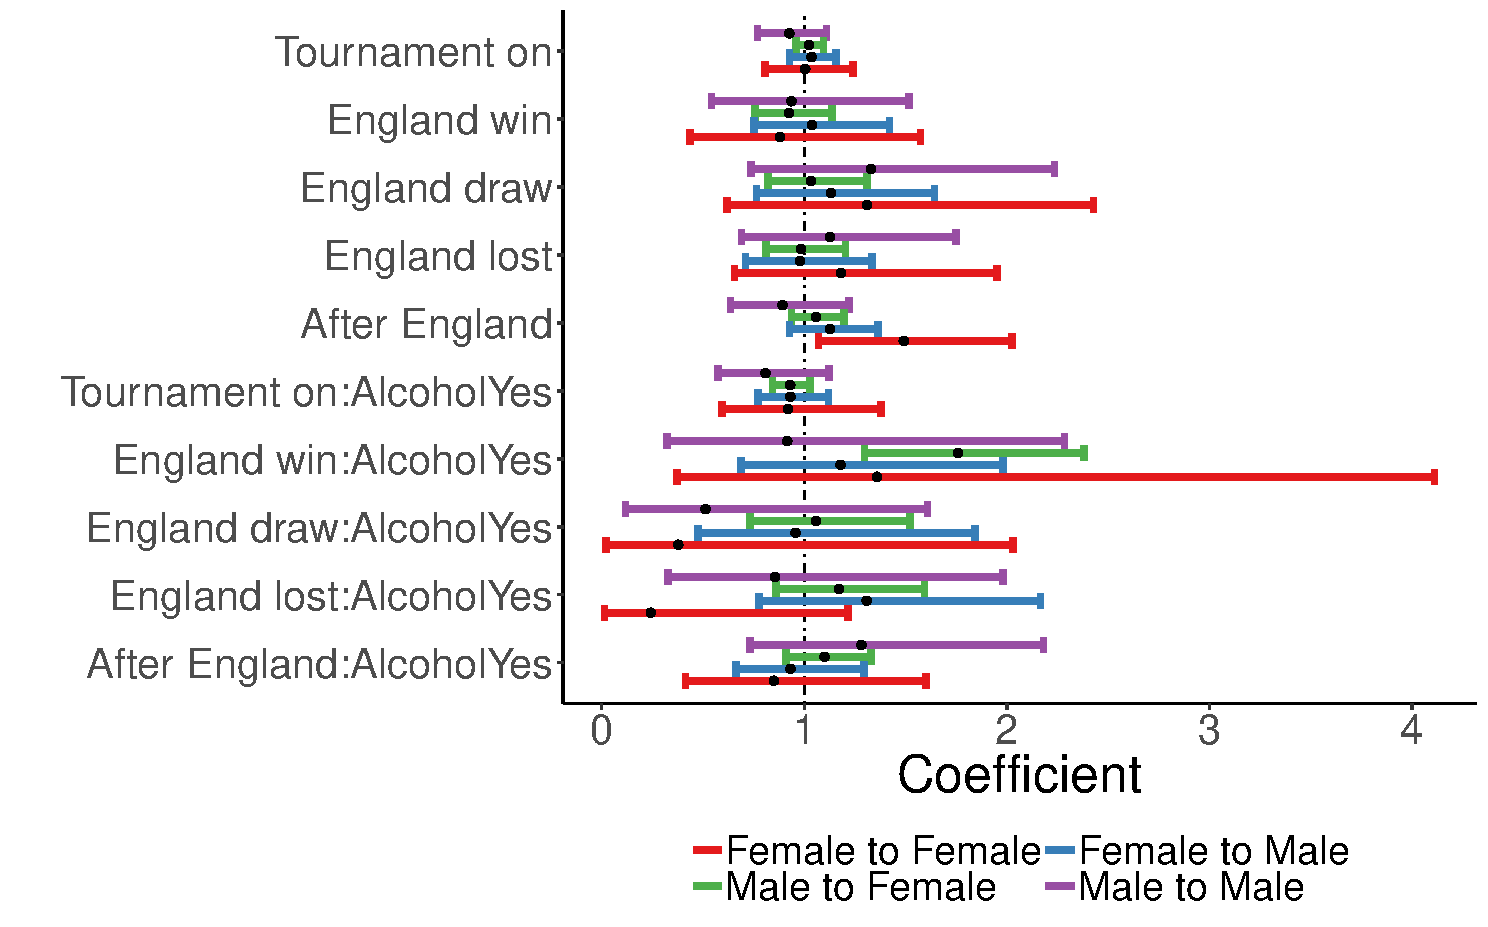
\includegraphics[width=1\textwidth]{DA_gender_compare.pdf}
\label{fig:DA_compare}
\end{figure}

\newpage

\subsection{How does the effect on DA compare to other types of crimes?}


\begin{figure}[htb!]
\centering
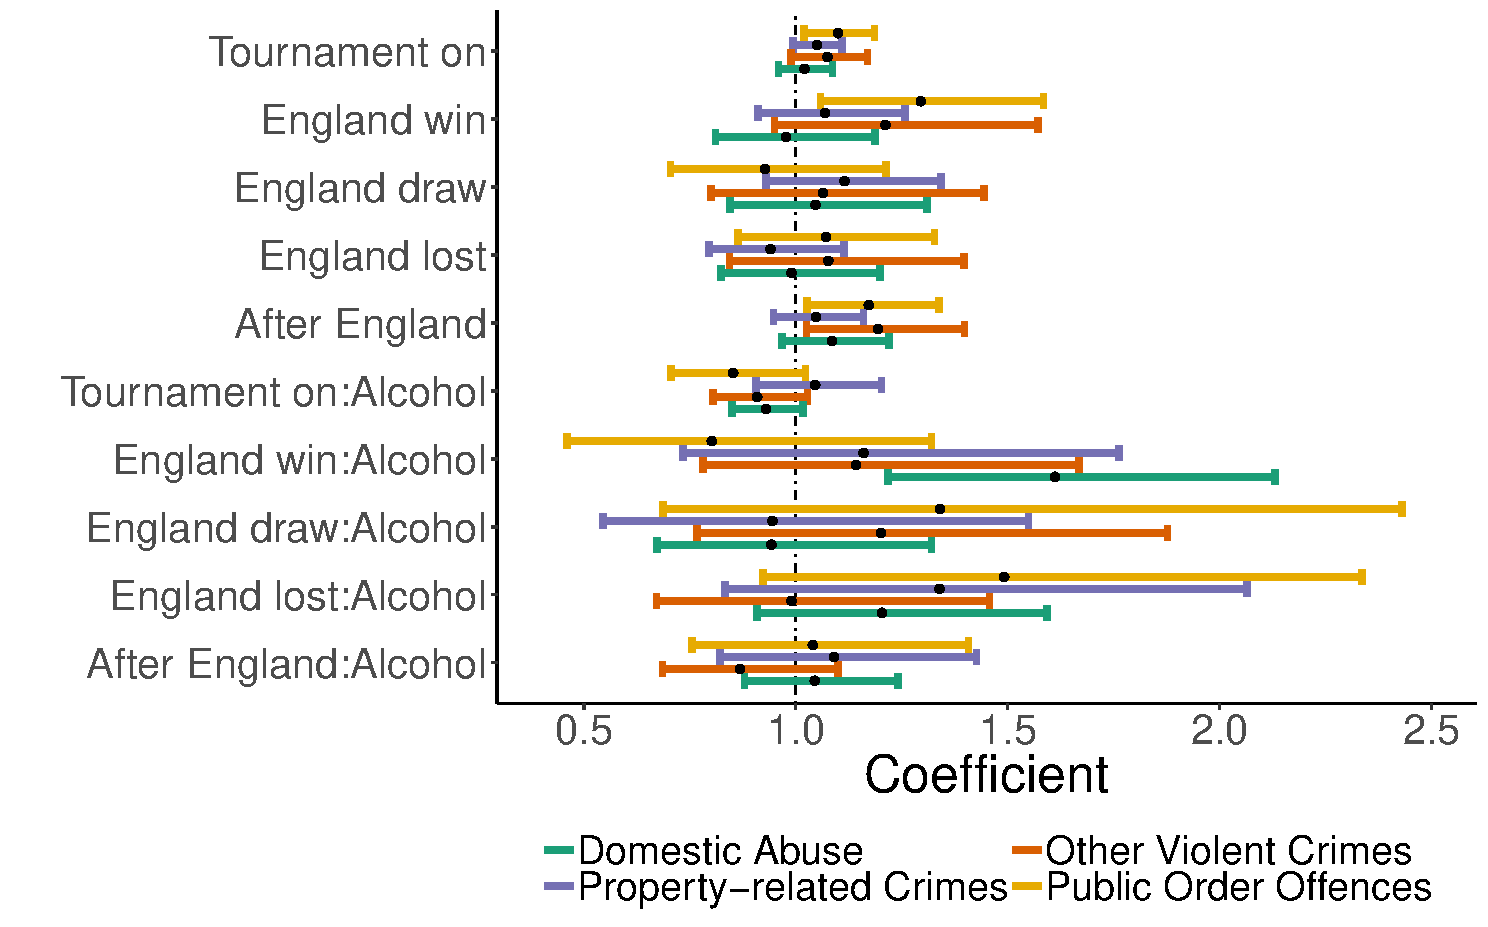
\includegraphics[width=1\textwidth]{DA_compare.pdf}
\label{fig:DA_compare}
\end{figure}

\newpage

\subsection{What can we say about the temporal dynamics of the effect?}
\begin{figure}[htb!]
\centering
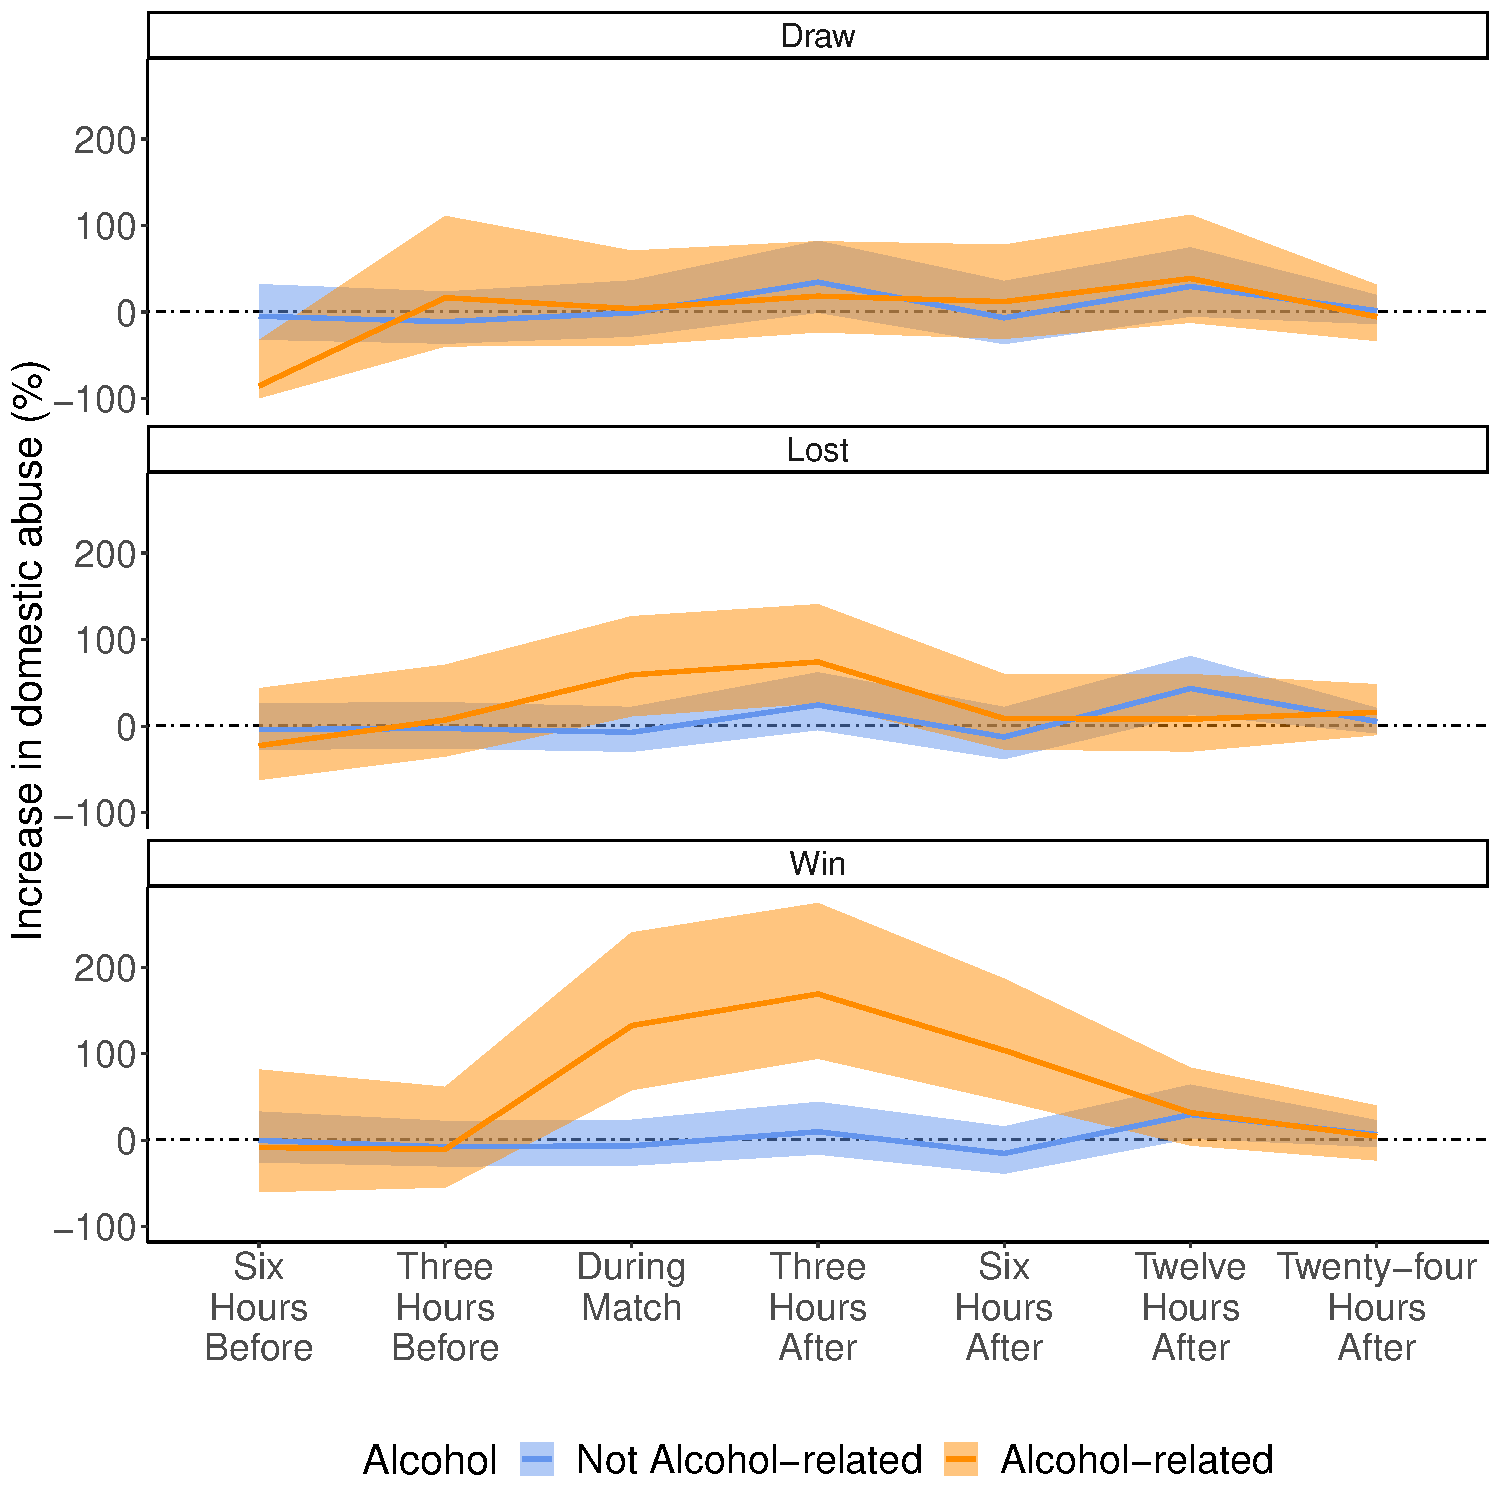
\includegraphics[width=1\textwidth]{Threehours.pdf}
\label{fig:DA_compare}
\end{figure}

\newpage

\subsection{What can we say about repeat incidents that are "triggered" on match days?}




\subsection{Reconciling with previous evidence}

So how can our results be reconciled with those reported previously? Card \& Lee have found an increase in domestic abuse when there is an unexpected loss, but not when the team wins (double check with Neil). An even more striking difference between our results is that they did not find any differential effect on alcohol-related incidents, whereas in our data, the effect is clearly only present in alcohol-related domestic abuse incidents. This discrepancy highlights that the effect on sports-induced emotional cues on domestic abuse are highly sensitive to the cultural context.

As expected, our findings are somewhat easier to reconcile with the results of other, England-based studies. Biricombe and Cafe found an approximately equal increase in domestic abuse when England lost or won, and no increase when they draw. In line with this, our results suggest that there is no increase when England draws - possibly due to the fact that only group-stage, relatively unimportant matches can result in a draw - but we also found an asymmetric effect of losses and wins. Kirby also reported an asymmetric effect, with a 38\% [15 - 66] and 26\% [13 - 40] increase when England lost or win or draw, respectively. However, upon re-analysing their data with separate coefficients for win and draw, and adding a month control, the effects change slightly, indicating a 46\% [29 - 65] increase when England wins, and a 33\% [10 - 59] increase when they lose, respectively, and no effect when they draw. This is more in line with our results, which suggest that while both losses and wins increase rates of domestic abuse, wins have a slightly more pronounced effect. Our results suggests that this asymmetric effect might be down to a large increase in alcohol-related incidents caused by an England victory.


But what kind of abuse? useful framework is the typology by Johnson (2008). Can we differentiate SCV and intimate terrorism by the time of reporting? We'd expect loads of CSV in our dataset and not much intimate terrorism (Johnson argues we should use ex partners dataset to investigate this due to the reporting bias in different types of domestic abuse). Intimate terrorism is characterised by harassment and stalking after separation. The big difference between SCV and IT is CONTROL. 


%\href{https://tavistockrelationships.ac.uk/policy-research/policy-briefings/914-couples-with-situational-violence}{Very useful classification}.


\subsection{Limitations}
underreporting, other factors like weather, campaigns may have increased willingness to report? issues about defining initimate partner violence, maybe increase because people celebrate outside? no.
If he had enough data, we could test for the same thing Card \& Lee have done.


\section{Conclusion}

context - increase in alcohol-related incidents when E wins is 62\%, NYE - 37\%, XMAS - 76\%, Friday - 28\%, Saturday - 102\%, Sunday - 94\%


\section{Appendix}

main findings:

60\% increase in alcohol-related da on days when E won

that comes from male to female

DA is different from other types of crimes

time course

miscell:

1) sensitivity of the result

2) comparison with rugby 

3) no effect of deprivation

4) sexual, vulnerable adult?

5) NOT more violent on england win days (taking into account that alcohol related incidents are more likely to be serious)/ no evidence for fewer control types/ no evidence that one-off cases are more likely to occur on E win days/ they are also not more likely to be reported sooner/later

6) Alcohol transition: equally from previously alcohol and non-alcohol related

7) On E wins days, alcohol related case increase comes from both new and old incidents

8) On E win days, incidents are not more/less likely to be public-private

9) Considering repeat incidents reoccurring as alcohol-related incidents on E win days, they are not more likely to be non or alcohol-related previously

10) Considering repeat incidents reoccurring on E win days, they are not more/less likely to have a long/short time elapsed since last/til next


%\bibliographystyle{naturemag}

\newpage

%\bibliography{football_refs}

\printbibliography
\end{document}
